\documentclass[11pt,a4paper]{article}
\usepackage[utf8]{inputenc}
\usepackage[T1]{fontenc}
\usepackage{amsmath,amssymb}
\usepackage{booktabs}
\usepackage{graphicx}
\usepackage{hyperref}
\usepackage[margin=25mm]{geometry}
\usepackage{caption}
\usepackage{float}
\usepackage{array}
\usepackage{xcolor}

\graphicspath{{../../official_extra_analysis/}}
\hypersetup{colorlinks=true,linkcolor=blue!60!black,citecolor=green!50!black,urlcolor=blue!70!black}
\setlength{\parskip}{0.45em}
\setlength{\parindent}{0pt}
\sloppy

\title{Supplementary Experimental Report:\\
       Raw-Frame Analysis, Anchor Lower-Trim Experiment,\\
       and Phase Center Sensitivity\\[5pt]
       \large Erlangen 28-May-2026 V5 Campaign -- Additional Analysis}
\author{Zekai Xiao\\
        OLAO Health GmbH / LMU Muenchen}
\date{June 2026}

\begin{document}
\maketitle
\tableofcontents
\newpage

\section{Context}

This document supplements the original English Vicon validation report and records the experiments that were completed after that report was sent for review. The original campaign left a central paradox: the V5 common-mode anchor layout corrected the anchor-side metric scale, with Sim3 scale moving from 0.958 for V4 to 1.010 for V5, yet the older V4 layout still gave the lower p50 static median on the same 24-position Erlangen campaign. In the transfer matrix, V4+C\_V4+D\_LOO gives 57.9 mm median 3D error, while V5+C\_V5+D\_LOO gives 67.8 mm. Those values are reproduced from \texttt{FULL\_V5\_scale\_to\_vicon/tables/v5\_vs\_v4\_scale\_comparison.csv} and \texttt{FULL\_transfer\_matrix/tables/transfer\_matrix\_48cells.csv}.

The additional experiments were designed to test whether this paradox is caused by delay--layout coupling rather than by a simple V4/V5 implementation error. The phase-center sensitivity analysis asks whether Vicon marker offsets can overturn the ranking. The raw-frame campaign uses the stored per-frame tag-anchor distributions to reduce positive NLOS tails. The anchor lower-trim blind experiment asks whether the same lower-tail statistic should also be used for inter-anchor self-calibration. The solver audit records which parts of the V1--V5 and T1--T4 solvers are actually algorithmic changes and which parts are preprocessing or policy changes.

The main conclusion is narrower and stronger than an accuracy claim. V5 is the physically better anchor geometry by metric scale, while V4 is the p50 single-environment positioning winner. When the positive tag-anchor range tail is reduced in static batch mode, the empirical ranking flips: V5 reaches 44.5 mm LOO, whereas the best V4 geometry row in the same raw-frame ranking is 53.9 mm. This flip is the strongest causal evidence that V4's p50 advantage came from beneficial cancellation between a distorted layout and structured positive range bias.

\section{Phase Center Sensitivity Analysis}

The phase-center sensitivity batch addressed a necessary alternative explanation. Vicon marker centers are not guaranteed to coincide with UWB antenna phase centers, and a systematic marker-to-antenna offset could make a geometrically correct UWB layout appear worse against the optical reference. The analysis therefore perturbed phase centers and repeated the relevant ranking checks rather than assuming that the marker geometry was exact.

The global shift sweep found that the V4-over-V5 p50 static ranking does not flip for tested offsets up to more than 10 mm. The manufacturing-variation Monte Carlo used 5000 samples per sigma level and found that $P(\mathrm{V4\ beats\ V5})$ remains at least 0.998 through $\sigma=8$ mm. The Vicon oracle rank is less stable: the table reports a fragile threshold around 2 mm for the oracle rank or worst-status conclusion. The cancellation valley itself remained invariant to the tested phase-center offsets, which means that the delay--layout coupling result is not an artifact of one exact optical marker model.

\begin{table}[H]
\centering
\caption{Phase-center robustness summary. Values are reproduced from \texttt{FULL\_V5\_phase\_center\_sensitivity/tables/a6\_robustness\_summary.csv}.}
\label{tab:phase_center}
\small
\begin{tabular}{@{}p{48mm}p{42mm}p{34mm}p{26mm}@{}}
\toprule
Conclusion & Baseline value & Flip threshold & Robustness \\
\midrule
V5 Sim3 scale $>$ 0.99 & 1.010 & $>$10 & robust \\
V4+LOO beats V5+LOO & V4-V5=-23.0 mm & $>$10 & robust \\
Vicon oracle rank/worst status & rank=2, worst=False & 2.0 & fragile \\
D\_tag LOO approximately 49.6mm & 49.028 mm; sensitivity 0.190 mm/mm & not binary & stable \\
D\_tag per-height spread V5 $<$ V4 & 7.4 $<$ 11.8 mm from prior mechanism audit & not directly flipped by global phase-center sweep & not directly tested here; use A4 as caveat \\
Cancellation valley exists & max tested operating-point valley-distance shift 11.37 & does not depend on absolute phase-center offset & invariant mechanism \\
\bottomrule
\end{tabular}
\end{table}

\begin{figure}[H]
\centering
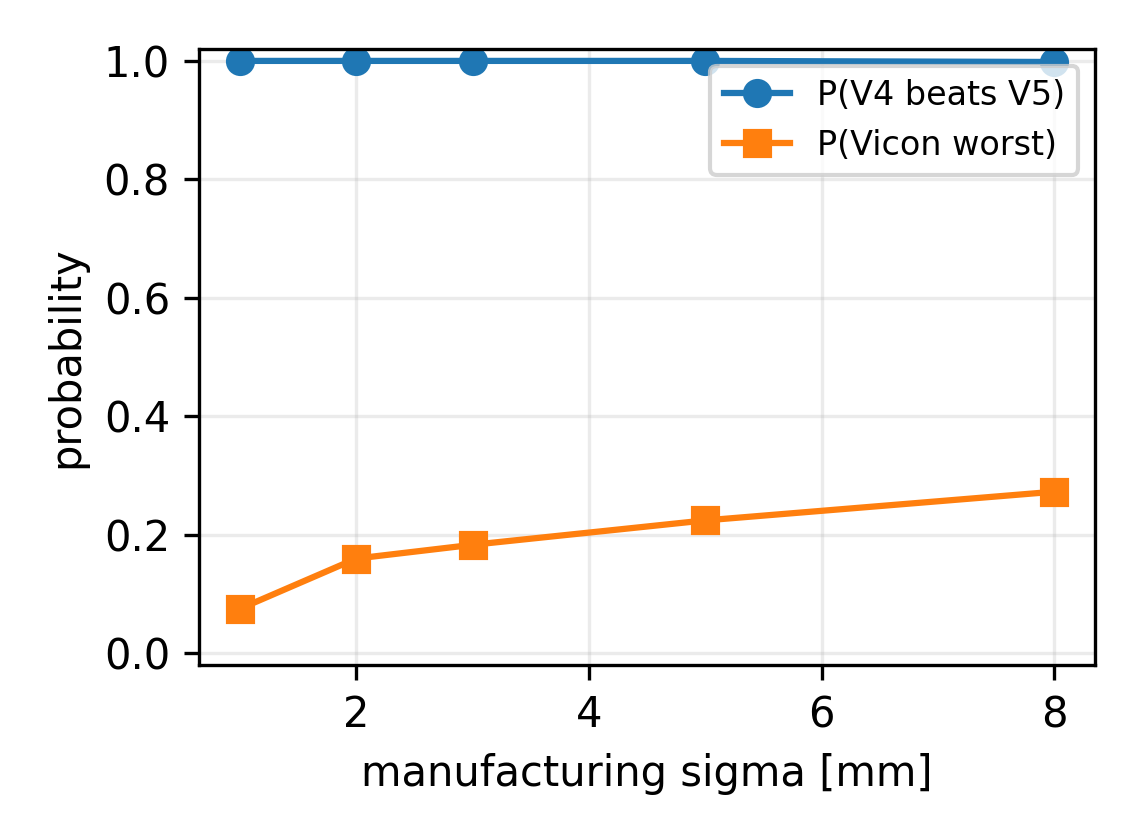
\includegraphics[width=0.88\textwidth]{FULL_V5_phase_center_sensitivity/figures/a2_ranking_probability_vs_sigma.png}
\caption{Manufacturing-variation phase-center Monte Carlo. The static V4-over-V5 p50 ranking is robust across the tested perturbation range, while the Vicon oracle rank is more fragile. Source: \texttt{FULL\_V5\_phase\_center\_sensitivity/figures/a2\_ranking\_probability\_vs\_sigma.png}.}
\label{fig:phase_mc}
\end{figure}

\section{Raw-Frame Range Distribution Analysis}

The raw-frame campaign began with a data-availability check. The static captures contain the raw per-frame tag-anchor observations needed for distribution-level analysis: 230,544 raw rows, 228,265 valid rows, and approximately 1200 frames per position-anchor link. This matters because the historical p50 pipeline collapses each link histogram to one median value before solving. If the histogram has a positive NLOS tail, a lower-quantile statistic can move the measurement closer to the LOS-side component without using CIR data.

\begin{table}[H]
\centering
\caption{Raw-frame campaign key numbers. Values are from \texttt{FULL\_V5\_experimental\_report/tables/rawframe\_v3\_key\_results.csv}.}
\label{tab:raw_key}
\begin{tabular}{@{}lrl@{}}
\toprule
Metric & Value & Unit \\
\midrule
Raw rows & 230544.0 & rows \\
Valid rows & 228265.0 & rows \\
Full grid configurations & 107448.0 & rows \\
Best honest LOO median & 44.5 & mm \\
Oracle lower bound & 44.6 & mm \\
Bootstrap CI & [33.4, 82.8] & mm \\
\bottomrule
\end{tabular}
\end{table}

The important result is the ranking flip. Under p50 aggregation, V4 wins the static LOO comparison despite having the wrong metric scale. Under lower-quantile static batch aggregation, V5 becomes the best geometry: lower\_trim\_20 with V5 and Huber30 gives 44.5 mm median LOO, while the best V4 geometry row in the same honest raw-frame ranking is 53.9 mm and the best Vicon geometry row is 44.7 mm. The oracle lower bound in the v3 ladder is 44.6 mm, so the V5 lower-tail row nearly reaches the recoverable median implied by the available raw distributions.

This is not presented as a new NLOS detection method. The lower-tail statistic is deliberately simple. Its value is experimental: it reduces the positive tag-anchor tail enough to remove the cancellation condition under which V4 was winning. The intervention therefore supports the mechanism claim that single-environment positioning accuracy can prefer a physically wrong geometry when the wrong geometry cancels structured range bias.

\begin{figure}[H]
\centering
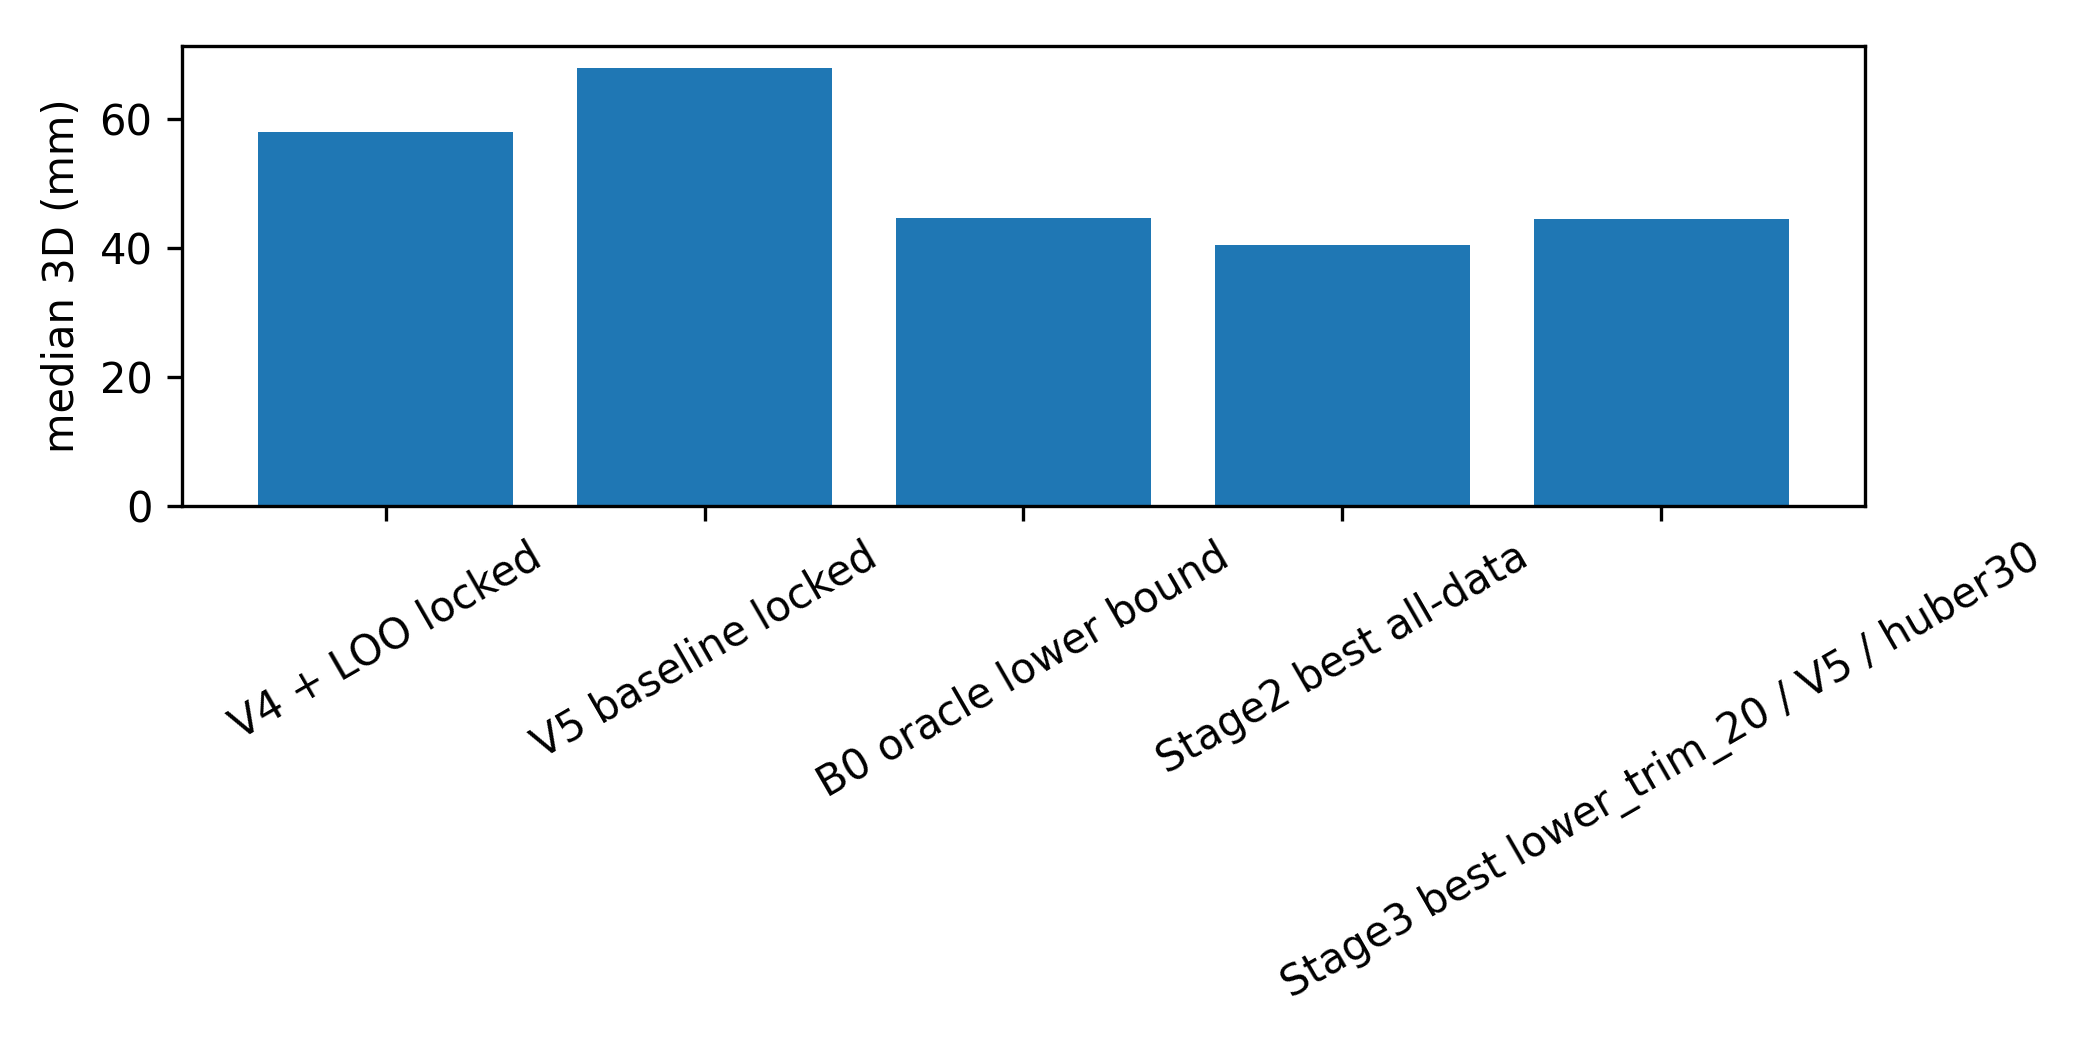
\includegraphics[width=0.88\textwidth]{FULL_V5_rawframe_bruteforce_v3/figures/s6_accuracy_ladder.png}
\caption{Raw-frame accuracy ladder. The lower-quantile V5 static batch row approaches the oracle median, while the tail remains unresolved. Source: \texttt{FULL\_V5\_rawframe\_bruteforce\_v3/figures/s6\_accuracy\_ladder.png}.}
\label{fig:raw_ladder}
\end{figure}

The caveat is the tail. The lower-quantile V5 row improves the median to 44.5 mm but keeps P95 at 164.1 mm and RMSE at 81.5 mm. By contrast, V4+C\_V4+D\_LOO under p50 has P95 110.6 mm. The lower-tail result therefore solves the typical static error better than it solves worst-case static positioning. The 5000-iteration bootstrap interval, 33.4--82.8 mm, also remains wide because the campaign has only 24 static positions.

\section{Anchor Lower-Trim Blind Experiment}

The raw-frame tag-anchor result raised a second question: if lower-tail statistics recover a better LOS-side tag-anchor range, should the same statistic be used for inter-anchor self-calibration? The blind anchor lower-trim experiment tested this directly by rebuilding V5-style anchor layouts with several inter-anchor aggregation methods and e\_i settings, then replaying the tag positioning pipeline.

The answer was negative. The inter-anchor distributions contain 56,000 valid rows across 28 pairs, with a median of 2000 frames per pair. Their mean skewness is 0.063, which is close to symmetric, while the mean p50 minus lower\_trim\_20 difference is 32.9 mm. In other words, lower\_trim\_20 systematically shortens the inter-anchor distances even though those distributions do not show the same right-tail structure as the static tag-anchor histograms.

\begin{table}[H]
\centering
\caption{Anchor lower-trim blind-experiment key numbers. Values are from \texttt{FULL\_V5\_experimental\_report/tables/anchor\_lower\_trim\_key\_results.csv}.}
\label{tab:anchor_lower_trim}
\begin{tabular}{@{}lrl@{}}
\toprule
Metric & Value & Unit \\
\midrule
AA valid rows & 56000.0 & rows \\
Median frames per pair & 2000.0 & frames \\
Mean skewness & 0.063 & skewness \\
Mean p50 - lower\_trim\_20 & 32.9 & mm \\
Best lower\_trim\_20 anchor row & 46.4 & mm LOO \\
Current p50 control & 44.5 & mm LOO \\
Best p50 e\_i=0 row & 43.2 & mm LOO \\
P(new wins), e\_i=0 & 0.659 & probability \\
\bottomrule
\end{tabular}
\end{table}

\begin{figure}[H]
\centering
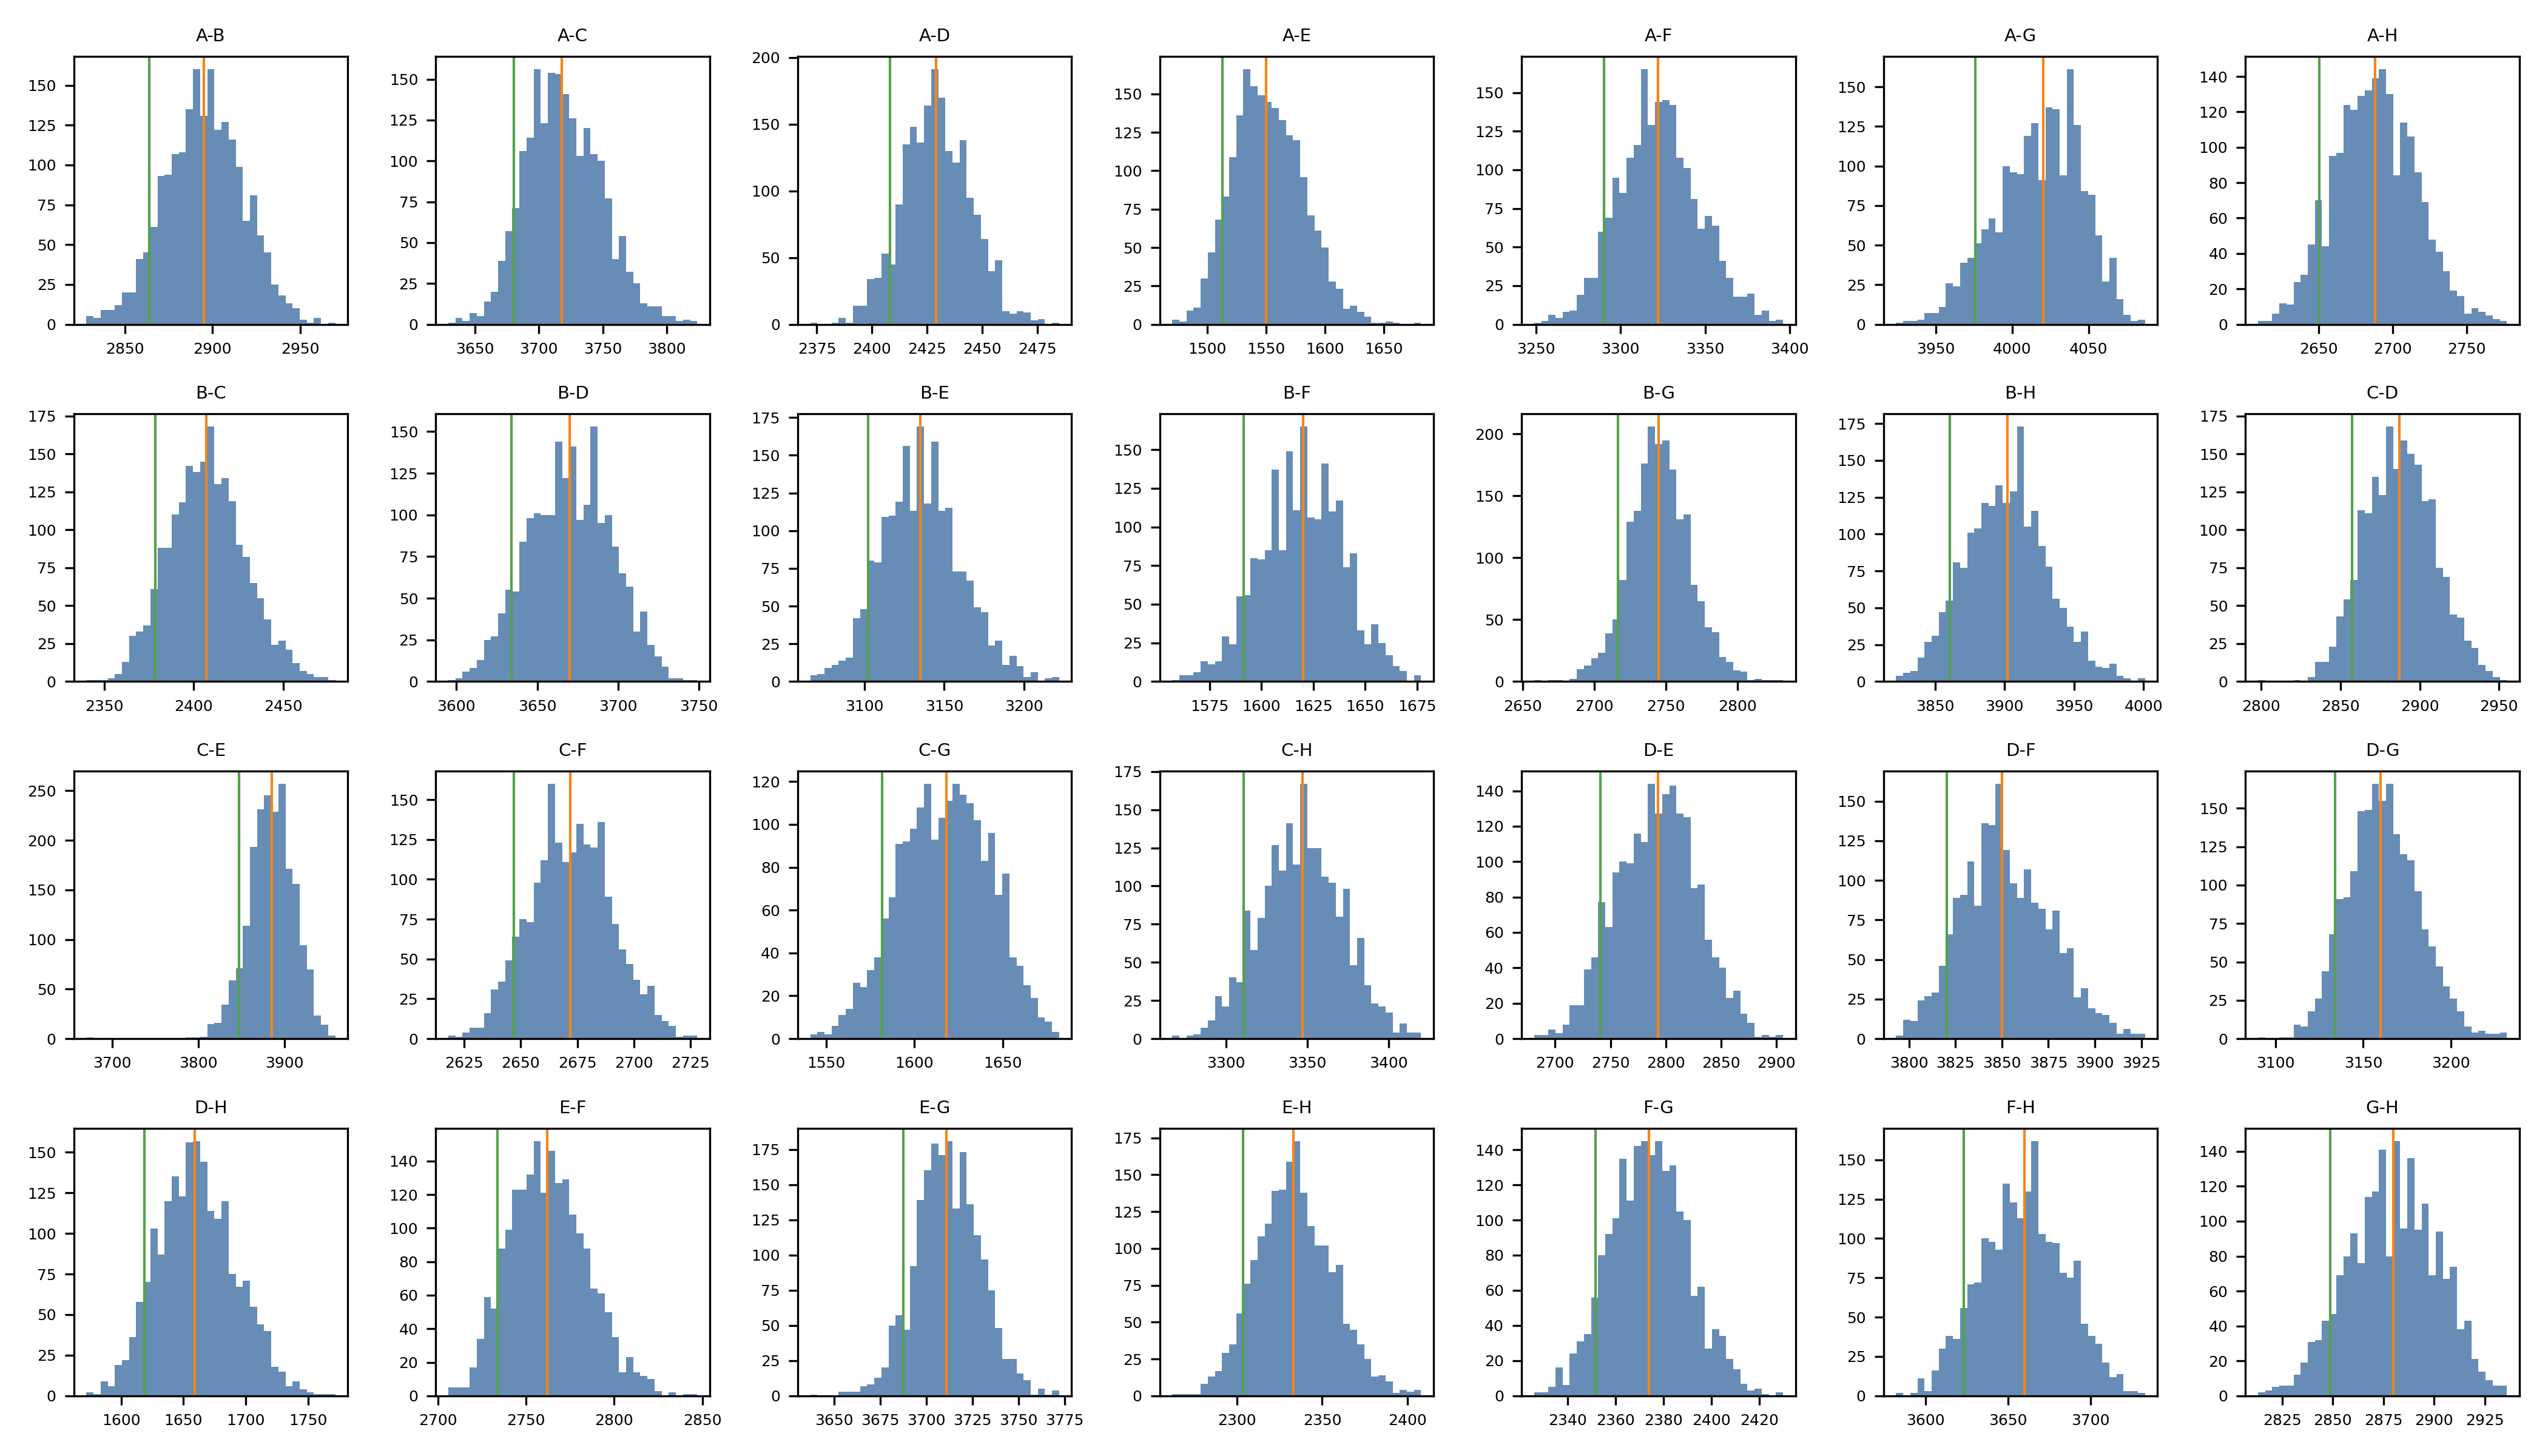
\includegraphics[width=0.88\textwidth]{FULL_V5_anchor_lower_trim/figures/l1_inter_anchor_histograms.png}
\caption{Inter-anchor raw range histograms. The near-symmetric distributions explain why lower-tail inter-anchor aggregation introduces a downward range bias rather than removing a positive tail. Source: \texttt{FULL\_V5\_anchor\_lower\_trim/figures/l1\_inter\_anchor\_histograms.png}.}
\label{fig:aa_hist}
\end{figure}

\begin{figure}[H]
\centering
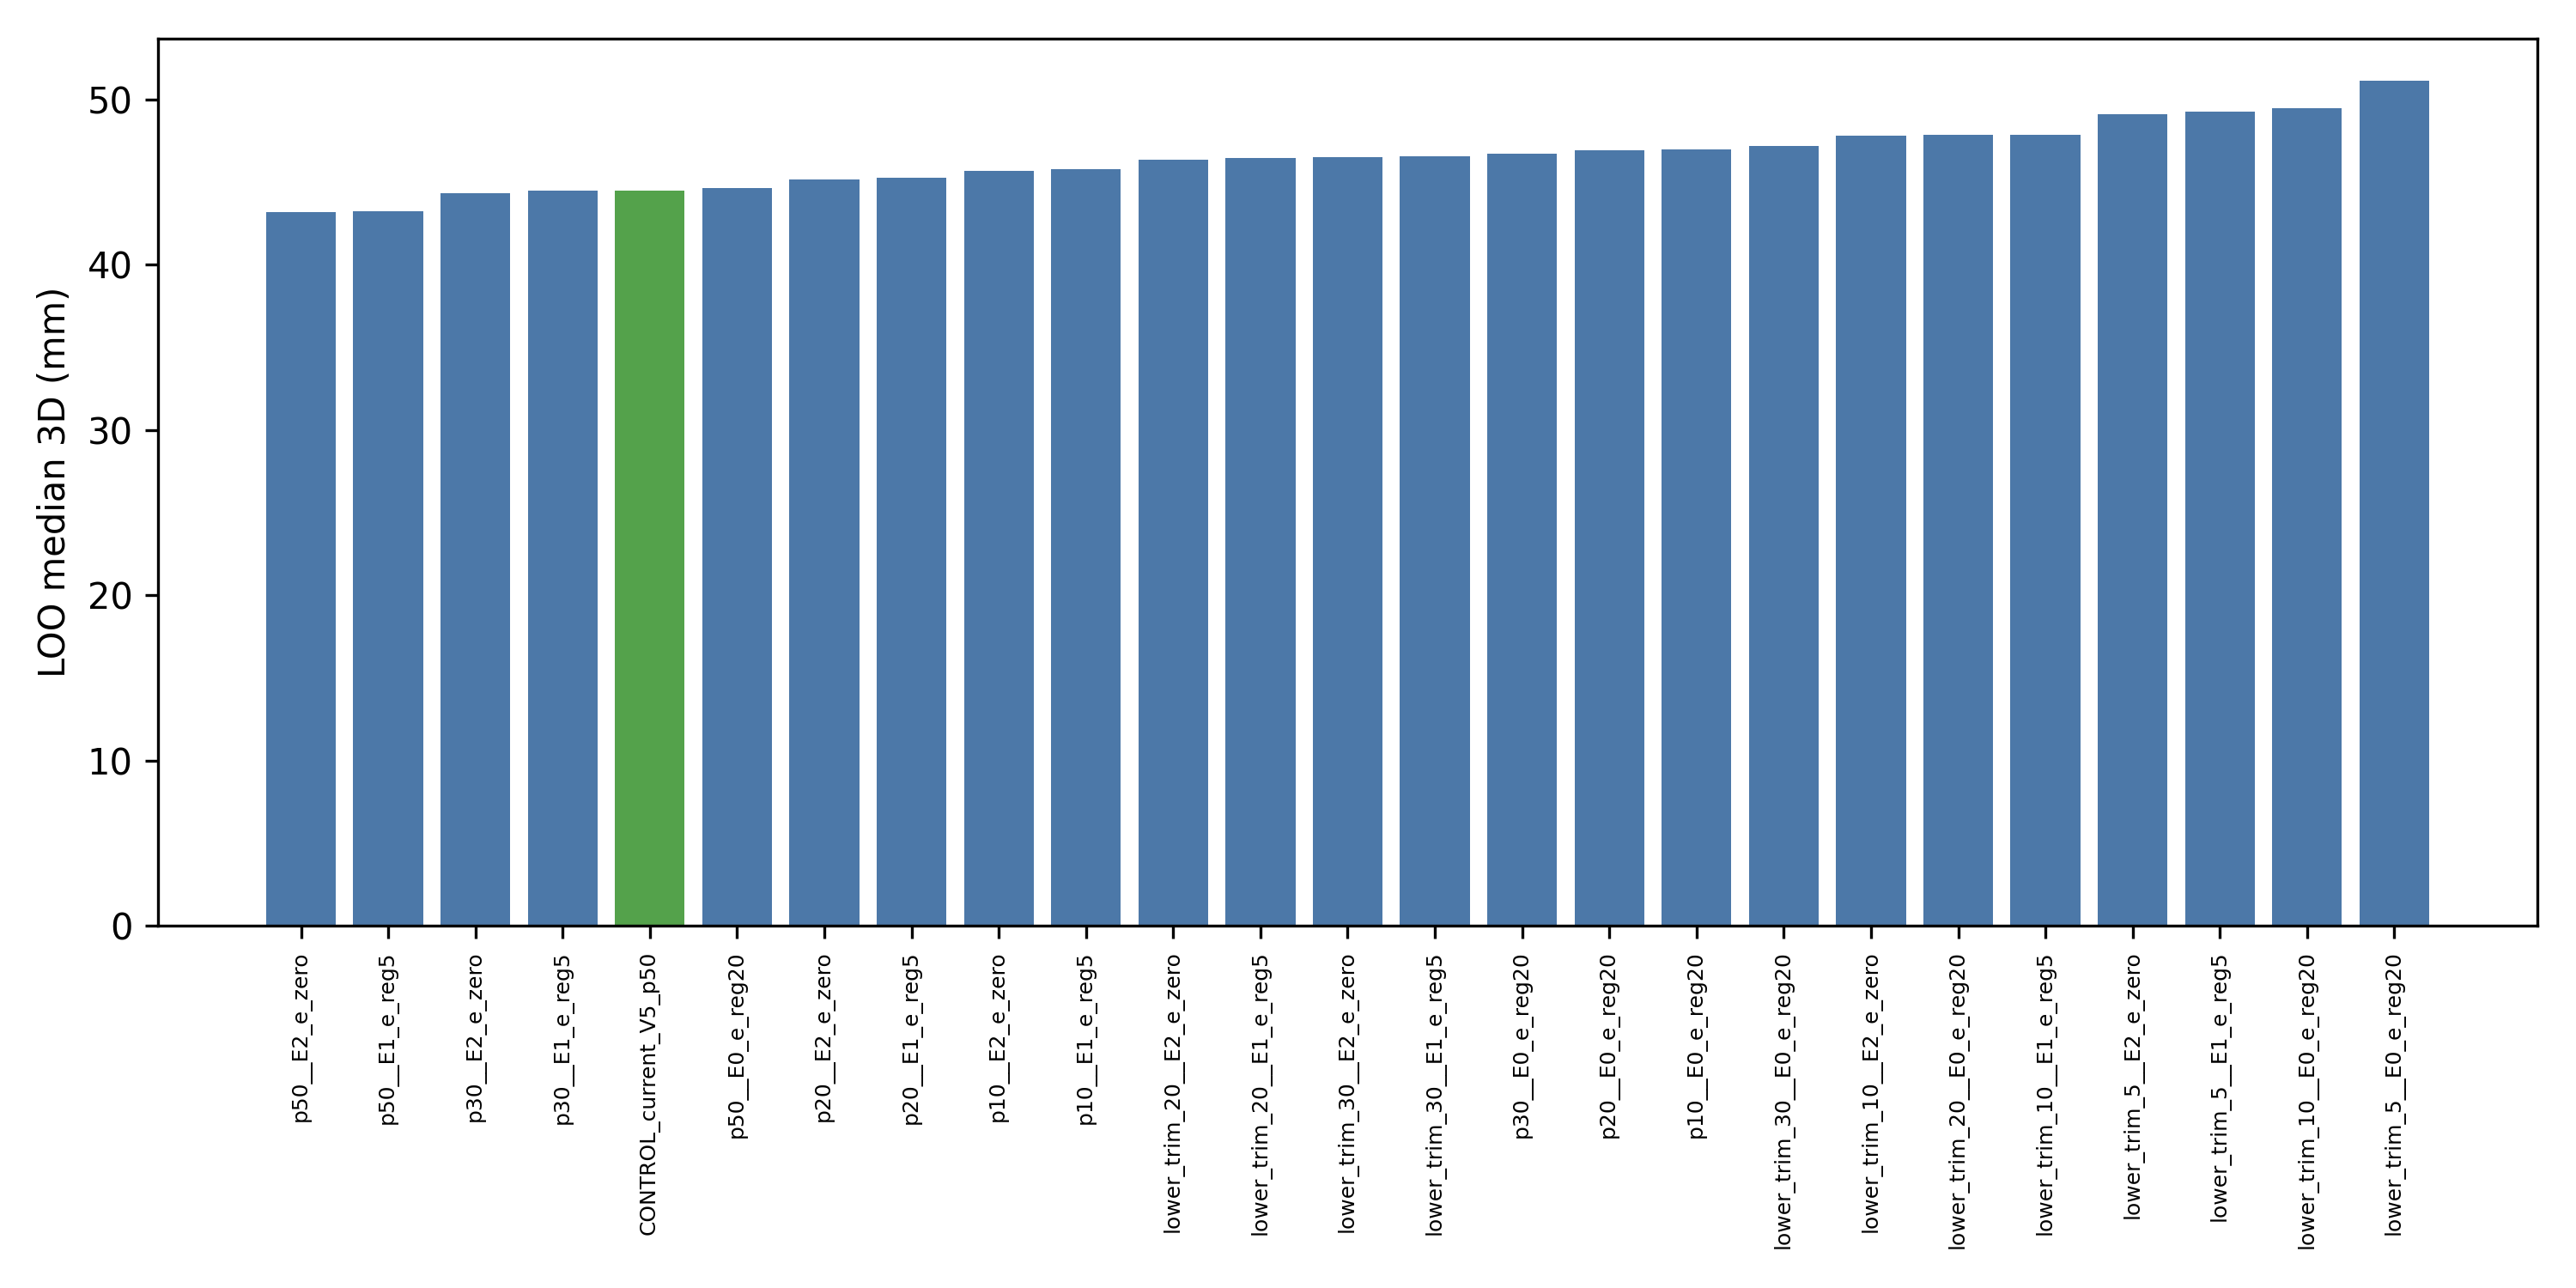
\includegraphics[width=0.88\textwidth]{FULL_V5_anchor_lower_trim/figures/l3_accuracy_by_anchor_method.png}
\caption{Blind anchor-aggregation comparison. The best lower\_trim\_20-anchor row is worse than the p50 control, while p50 with e\_i=0 is a small, not yet statistically locked, candidate improvement. Source: \texttt{FULL\_V5\_anchor\_lower\_trim/figures/l3\_accuracy\_by\_anchor\_method.png}.}
\label{fig:anchor_method}
\end{figure}

The practical rule from this experiment is simple: keep p50/median for inter-anchor self-calibration in this dataset, and treat lower-quantile aggregation as a tag-anchor static batch estimator. The e\_i result is separate. p50 with e\_i=0 reaches 43.2 mm LOO, compared with 44.5 mm for the current p50/e\_reg20 control, but the paired bootstrap gives $P(\mathrm{new\ wins})=0.659$ and a confidence interval crossing zero. This is a candidate setting for the next capture, not a locked replacement.

\section{Solver Audit Summary}

The solver audit found five core anchor-layout solver generations and four C-level tag solver versions, plus one Python tag-solver policy variant. The audit matters because several campaign results are preprocessing or parameterization effects rather than new numerical solvers. In particular, no production T5 tag solver was found; the lower-trim and Huber30 improvements are changes to range aggregation and loss configuration around the existing tag-solver family.

\begin{table}[H]
\centering
\caption{Anchor solver evolution from the read-only audit. Source: \texttt{../../../../Analysis/solver\_audit/reports/SOLVER\_AUDIT\_SUMMARY.md}.}
\label{tab:anchor_solver}
\small
\begin{tabular}{@{}p{27mm}p{70mm}p{45mm}@{}}
\toprule
Version & One-line description & Delay model or key parameter \\
\midrule
V1 / v1-old & early MDS baseline & no delay \\
V2 & inverse-variance bidirectional fusion & no delay \\
V3-lite & median/MAD/MVUE fusion & no delay \\
V3-full & robust fusion plus alternating per-anchor delays & per-anchor delays \\
V4 / v4-io & bounded independent-delay Huber inter-anchor solve & dA=0, [-60,+60] mm \\
V5 / common-mode & common-mode extension, di=c+ei & c=111.985 mm, e\_reg=20 mm artifact \\
\bottomrule
\end{tabular}
\end{table}

\begin{table}[H]
\centering
\caption{Tag solver evolution from the read-only audit. Source: \texttt{../../../../Analysis/solver\_audit/reports/SOLVER\_AUDIT\_SUMMARY.md}.}
\label{tab:tag_solver}
\small
\begin{tabular}{@{}p{28mm}p{80mm}p{36mm}@{}}
\toprule
Version & One-line description & Status \\
\midrule
T1 & robust WLS multilateration & current method default \\
T2 & T1 plus quality-aware sigma inflation & C method 2 \\
T3 & T2 plus residual EMA and temporal prior & C method 3 \\
T4 & adaptive full-anchor T1 / low-redundancy T3 policy & Python wrapper plus C method 4 \\
T4\_V6\_IMU\_GATE & T4 plus accelerometer-gated temporal prior & policy variant \\
\bottomrule
\end{tabular}
\end{table}

The current research configuration is V5 common-mode self-calibration with the existing artifact at $c=111.985$ mm and e\_reg20, combined with a tag solver that defaults to robust WLS and Huber scale 30 mm after recent edits. The audit recommends keeping p50 inter-anchor aggregation, testing lower-tail tag-side aggregation for static batch operation, explicitly labeling e\_i settings, and fixing the C-core loss-selector mismatch where the Python interface exposes a linear option but C validation resets it to Huber.

\section{Updated Headline Table}

The headline table below is reproduced from \texttt{FULL\_V5\_experimental\_report/tables/locked\_headline\_v2.csv}. It should be read as a campaign registry rather than a single leaderboard, because rows differ in evaluation protocol. Rows labelled in-sample, diagnostic, Sim3, or oracle should not be used as deployment claims. Row O is the new raw-frame static batch result; its median is strong, but its P95 is not.

\begin{table}[H]
\centering
\caption{Updated locked headline table. Empty cells indicate metrics not reported for that row in the source table.}
\label{tab:headline}
\scriptsize
\begin{tabular}{@{}cp{38mm}p{17mm}p{15mm}p{15mm}p{38mm}c@{}}
\toprule
Row & Variant & Median & P95 & RMSE & Evaluation & New \\
\midrule
A & V4 production & 71.9 & 176.0 & 110.4 & in-sample, all 24 &  \\
B & V4 + D\_LOO & 57.9 & 110.6 & 74.4 & LOO-CV &  \\
C & V5 baseline & 67.8 & 160.5 & 86.4 & LOO-CV &  \\
D & V5 apparent best & 56.0 & 143.1 & 79.5 & in-sample post-selected &  \\
E & V4 apparent best & 54.9 & 154.8 & 79.6 & in-sample post-selected &  \\
F & V5 corrected & 65.6 &  &  & OOB-bootstrap &  \\
G & V4 corrected & 64.5 &  &  & OOB-bootstrap &  \\
H & V5 bootstrap CI & [54.3, 63.7] &  &  & bootstrap 95\% CI &  \\
I & Nested CV (height) & 82.9 &  &  & held-out test &  \\
J & Nested CV (quadrant) & 88.0 &  &  & held-out test &  \\
K & Nested CV (spatial6) & 94.2 &  &  & held-out test &  \\
L & ROTO V5 per-frame & 101.5 & 214.4 & 126.2 & BEST-FIT-ALIGNED &  \\
M & ROTO SE(3) aligned & 82.5 & 185.2 & 103.7 & diagnostic &  \\
N & ROTO Sim3 aligned & 74.3 & 160.8 & 94.8 & diagnostic only &  \\
O & lower\_trim\_20 + Huber30 + V5 & 44.5 & 164.1 & 81.5 & LOO-CV & YES \\
P & lower\_trim\_20 + Huber30 + V5(e\_i=0 anchor refit) & 43.2 & 163.1 & 81.8 & LOO-CV; anchor refit diagnostic & YES \\
Q & Oracle lower bound & 44.6 &  &  & oracle & YES \\
R & Bootstrap CI (lower\_trim\_20) & [33.4, 82.8] &  &  & bootstrap 95\% CI & YES \\
\bottomrule
\end{tabular}
\end{table}

The most important comparison is not Row O against every other row, but the ranking reversal under a controlled change in tag-anchor range bias. Under p50, V4 wins at 57.9 mm versus V5 at 67.8 mm. Under lower\_trim\_20 with Huber30, V5 reaches 44.5 mm and the best V4 raw-frame geometry row is 53.9 mm. That reversal is the evidence for delay--layout--NLOS coupling.

\section{Updated Claim Matrix}

The V3 report reorganizes the claim matrix around delay--layout coupling. The campaign-level counts are 10 Level A claims, 10 Level B claims, 5 Level C claims, and 2 Level D claims after removing the mixture-model ranking as a paper-level scientific claim and downgrading the lower-quantile method claim to a caveated engineering result. The full claim register remains in \texttt{FULL\_V5\_experimental\_report/tables/claim\_evidence\_matrix\_v2.csv}; the V3 narrative is the controlling interpretation where the prose and the raw CSV differ.

\begin{table}[H]
\centering
\caption{New or revised claims introduced by the raw-frame and anchor lower-trim work.}
\label{tab:new_claims}
\small
\begin{tabular}{@{}clp{112mm}@{}}
\toprule
ID & Level & Recommended wording \\
\midrule
26 & B & Lower-quantile tag-anchor aggregation improves static median when enough frames are accumulated, but the P95 remains high. \\
27 & A & Inter-anchor raw ranges are nearly symmetric; lower-tail aggregation is inappropriate for anchor self-calibration here. \\
28 & B & The e\_i=0 or low-e\_i V5 variant is slightly better for the raw-frame static estimator, but the bootstrap evidence is not decisive. \\
29 & A & When tag-anchor positive bias is reduced, V4's cancellation advantage disappears and V5 becomes the better geometry. \\
\bottomrule
\end{tabular}
\end{table}

The practical wording should stay conservative. Lower\_trim\_20 is a static batch extractor for this campaign, not a CIR-free NLOS detector. V5 transfer to new rooms remains untested. ROTO still has a dynamic floor around 101.5 mm under the conservative BEST-FIT-ALIGNED convention. The central paper claim is the mechanism: a physically wrong self-calibration can win in the same environment because its scale error cancels structured positive range bias.

\section{Engineering Recommendations}

For anchor self-calibration, use p50/median inter-anchor ranges in Erlangen-style captures. The inter-anchor distributions are nearly symmetric and lower-tail aggregation worsened the blind replay. The V5 common-mode family should be reported with its e\_i setting. The e\_i=0 and e\_reg5 variants are worth testing in the next campaign, but e\_reg20 should not be silently replaced on the basis of a 24-position bootstrap with $P(\mathrm{new\ wins})=0.659$.

For static tag solving, keep raw per-frame ranges and test lower-quantile aggregation when enough frames per link are accumulated. In this campaign, the useful row is ``V5 p50 anchors, lower\_trim\_20 tag ranges, Huber30, D\_tag LOO.'' The D\_tag value is estimator-specific: the p50 V5 LOO value is 49.621 mm, whereas the lower-quantile V5/Huber30 row calibrates around a much smaller effective tag delay. These numbers should not be mixed.

For dynamic operation, do not transfer the static lower-tail result directly to one-frame ROTO solves. ROTO remains a separate limitation, and the current conservative headline is 101.5 mm BEST-FIT-ALIGNED. The alignment audit and time-offset sweep should be reported as diagnostics, not as a solved dynamic-tracking pipeline.

For firmware and capture design, the priority is to keep saving raw per-frame ranges. The raw data already made the ranking-flip experiment possible. A future quasi-static mode can accumulate a short histogram only when IMU and range stability indicate that the tag is not moving, then compare p50 and lower-quantile solves within that window.

\section{Open Questions}

The first open question is tail reduction. The lower-quantile row improves the static median but leaves P95 around 164 mm. The next analysis should identify which positions and anchors cause this tail and whether per-anchor stability rules can reduce it without giving back the median gain.

The second open question is external validation. The current LOO and bootstrap results are still within one room and one 24-position campaign. A second-room run with a frozen pipeline should repeat p50 V4, p50 V5, lower-quantile V5, p50/e\_i=0 anchors, and the same hard validation splits.

The third open question is D\_tag self-calibration without known positions. The present D\_tag values depend on Vicon-supported static folds or known-position residuals. Deployment needs a small-calibration procedure that can estimate the appropriate device- and estimator-specific D\_tag without optical ground truth.

The fourth open question is dynamic transfer. Static lower-quantile aggregation requires a histogram, while ROTO has single-frame measurements. The next dynamic work should test quasi-static sliding windows, hardware time synchronization, and physical tag-orientation sweeps before claiming a real-time dynamic improvement.

\end{document}
